\documentclass[border=6pt]{standalone}
\usepackage{fontspec,unicode-math}
\setmainfont{Noto Serif}
\setmathfont{STIXTwoMath-Regular.otf}
\usepackage{tikz}
\usetikzlibrary{arrows.meta,calc,patterns,decorations.pathmorphing}
\tikzset{heavy/.style={line width=1.1pt,line cap=round,line join=round},
 fine/.style={line width=.58pt,line cap=round,line join=round},
 pale/.style={line width=.40pt},
 arr/.style={line width=.70pt,-{Latex[length=1.9mm,width=1.1mm]}},
 dim/.style={line width=.58pt,{Latex[length=1.55mm,width=.85mm]}-{Latex[length=1.55mm,width=.85mm]}},
 txt/.style={font=\fontsize{11}{13}\selectfont,inner sep=1.1pt},
 mini/.style={font=\fontsize{9}{11}\selectfont,inner sep=.9pt}}
\begin{document}
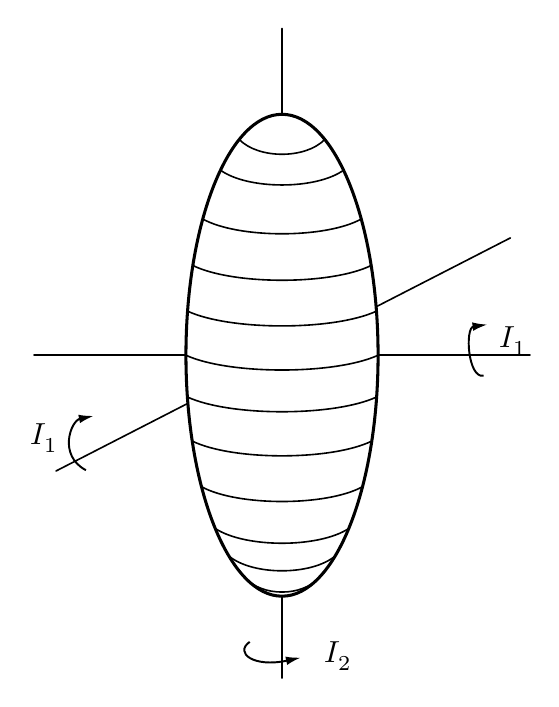
\begin{tikzpicture}[x=1cm,y=1cm,line join=round]
% Rear portions of three axes are deliberately obscured by the white body.
\draw[fine] (-3.15,0)--(3.15,0);
\draw[fine] (-2.87,-1.47)--(2.90,1.49);
\draw[fine] (0,-4.10)--(0,4.15);
\draw[heavy,fill=white] (0,0) ellipse[x radius=1.22,y radius=3.06];
\begin{scope}
 \clip (0,0) ellipse[x radius=1.22,y radius=3.06];
 % Eleven latitude arcs are front-visible projected circumferences.
 \foreach \yy in {-2.82,-2.55,-2.20,-1.67,-1.09,-.53,0,.56,1.14,1.73,2.35,2.74}{
  \pgfmathsetmacro{\rad}{1.22*sqrt(max(0,1-(\yy/3.06)^2))}
  \draw[fine] (-\rad,\yy) .. controls (-.55*\rad,\yy-.25) and (.55*\rad,\yy-.25) .. (\rad,\yy);
 }
\end{scope}
% Axis roll markers are outside the body, with deliberate gaps to the axes.
\draw[arr] (2.56,-.26) .. controls (2.36,-.30) and (2.32,.35) .. (2.61,.39);
\node[txt,anchor=west] at (2.72,.18) {$I_1$};
\draw[arr] (-2.49,-1.46) .. controls (-2.85,-1.27) and (-2.68,-.83) .. (-2.39,-.77);
\node[txt,anchor=east] at (-2.80,-1.05) {$I_1$};
\draw[arr] (-.41,-3.64) .. controls (-.61,-3.78) and (-.36,-3.97) .. (.24,-3.84);
\node[txt,anchor=west] at (.50,-3.82) {$I_2$};
\end{tikzpicture}
\end{document}
